% Options for packages loaded elsewhere
\PassOptionsToPackage{unicode}{hyperref}
\PassOptionsToPackage{hyphens}{url}
\PassOptionsToPackage{dvipsnames,svgnames,x11names}{xcolor}
%
\documentclass[
  10pt,
  ignorenonframetext,
]{beamer}
\usepackage{pgfpages}
\setbeamertemplate{caption}[numbered]
\setbeamertemplate{caption label separator}{: }
\setbeamercolor{caption name}{fg=normal text.fg}
\beamertemplatenavigationsymbolsempty
% Prevent slide breaks in the middle of a paragraph
\widowpenalties 1 10000
\raggedbottom
\setbeamertemplate{part page}{
  \centering
  \begin{beamercolorbox}[sep=16pt,center]{part title}
    \usebeamerfont{part title}\insertpart\par
  \end{beamercolorbox}
}
\setbeamertemplate{section page}{
  \centering
  \begin{beamercolorbox}[sep=12pt,center]{part title}
    \usebeamerfont{section title}\insertsection\par
  \end{beamercolorbox}
}
\setbeamertemplate{subsection page}{
  \centering
  \begin{beamercolorbox}[sep=8pt,center]{part title}
    \usebeamerfont{subsection title}\insertsubsection\par
  \end{beamercolorbox}
}
\AtBeginPart{
  \frame{\partpage}
}
\AtBeginSection{
  \ifbibliography
  \else
    \frame{\sectionpage}
  \fi
}
\AtBeginSubsection{
  \frame{\subsectionpage}
}
\usepackage{amsmath,amssymb}
\usepackage{lmodern}
\usepackage{iftex}
\ifPDFTeX
  \usepackage[T1]{fontenc}
  \usepackage[utf8]{inputenc}
  \usepackage{textcomp} % provide euro and other symbols
\else % if luatex or xetex
  \usepackage{unicode-math}
  \defaultfontfeatures{Scale=MatchLowercase}
  \defaultfontfeatures[\rmfamily]{Ligatures=TeX,Scale=1}
\fi
\usetheme[]{Singapore}
\usefonttheme{serif}
% Use upquote if available, for straight quotes in verbatim environments
\IfFileExists{upquote.sty}{\usepackage{upquote}}{}
\IfFileExists{microtype.sty}{% use microtype if available
  \usepackage[]{microtype}
  \UseMicrotypeSet[protrusion]{basicmath} % disable protrusion for tt fonts
}{}
\makeatletter
\@ifundefined{KOMAClassName}{% if non-KOMA class
  \IfFileExists{parskip.sty}{%
    \usepackage{parskip}
  }{% else
    \setlength{\parindent}{0pt}
    \setlength{\parskip}{6pt plus 2pt minus 1pt}}
}{% if KOMA class
  \KOMAoptions{parskip=half}}
\makeatother
\usepackage{xcolor}
\newif\ifbibliography
\usepackage{graphicx}
\makeatletter
\def\maxwidth{\ifdim\Gin@nat@width>\linewidth\linewidth\else\Gin@nat@width\fi}
\def\maxheight{\ifdim\Gin@nat@height>\textheight\textheight\else\Gin@nat@height\fi}
\makeatother
% Scale images if necessary, so that they will not overflow the page
% margins by default, and it is still possible to overwrite the defaults
% using explicit options in \includegraphics[width, height, ...]{}
\setkeys{Gin}{width=\maxwidth,height=\maxheight,keepaspectratio}
% Set default figure placement to htbp
\makeatletter
\def\fps@figure{htbp}
\makeatother
\setlength{\emergencystretch}{3em} % prevent overfull lines
\providecommand{\tightlist}{%
  \setlength{\itemsep}{0pt}\setlength{\parskip}{0pt}}
\setcounter{secnumdepth}{-\maxdimen} % remove section numbering
\ifLuaTeX
  \usepackage{selnolig}  % disable illegal ligatures
\fi
\IfFileExists{bookmark.sty}{\usepackage{bookmark}}{\usepackage{hyperref}}
\IfFileExists{xurl.sty}{\usepackage{xurl}}{} % add URL line breaks if available
\urlstyle{same} % disable monospaced font for URLs
\hypersetup{
  pdftitle={Teaching about Open and Reproducible Science},
  pdfauthor={Stefanie Muff},
  colorlinks=true,
  linkcolor={Maroon},
  filecolor={Maroon},
  citecolor={Blue},
  urlcolor={blue},
  pdfcreator={LaTeX via pandoc}}

\title{Teaching about Open and Reproducible Science}
\subtitle{An idea for a transferable skills course}
\author{Stefanie Muff}
\date{January 18th 2023}

\begin{document}
\frame{\titlepage}

\begin{frame}{Background}
\protect\hypertarget{background}{}
\(~\)

\begin{itemize}
\tightlist
\item
  In November 2022, Bob and I were involved in teaching a PhD course on
  \emph{Open and Reproducible Science}.
\end{itemize}

\vspace{2mm}

\begin{itemize}
\tightlist
\item
  2.5 credit points.
\end{itemize}

\vspace{2mm}

\begin{itemize}
\tightlist
\item
  Taking place in the Alpine center in Finse.
\end{itemize}

\vspace{2mm}

\begin{itemize}
\tightlist
\item
  Roughly 25 participants.
\end{itemize}
\end{frame}

\begin{frame}
We received very positive feedback from the students.

\vspace{4mm}

\begin{quote}

 "I think this course should be continued."
 
 \vspace{2mm}

 "There are many colleagues who love the idea of open science but they feel isolated nad do not have a direction to move ahead. I will recommend this course to them."
 
  \vspace{2mm}

 "I would recommend the course to all PhDs and post-docs at my department/collaborators"
 
 \vspace{2mm}
 
 "I hope that more young researchers can join the course in the future. I think the information and skills after such course can influence significantly someone's career or even change it."
 
  \vspace{2mm}
  
  Our students: "This course should be on offer as a transferable skills course at NTNU!" 

\end{quote}
\end{frame}

\begin{frame}
\begin{block}{Course content}
\protect\hypertarget{course-content}{}
\(~\)

\begin{itemize}
\tightlist
\item
  Introduction on terminology (open science, reproducibility,
  transparancy)
\end{itemize}

\vspace{1mm}

\begin{itemize}
\tightlist
\item
  Data Management Plan (DMP)
\end{itemize}

\vspace{1mm}

\begin{itemize}
\tightlist
\item
  Data collection and data handling
\end{itemize}

\vspace{1mm}

\begin{itemize}
\tightlist
\item
  Data repositories
\end{itemize}

\vspace{1mm}

\begin{itemize}
\tightlist
\item
  FAIR data principles
\end{itemize}

\vspace{1mm}

\begin{itemize}
\tightlist
\item
  Using version control (git/GitHub)
\end{itemize}

\vspace{1mm}

\begin{itemize}
\tightlist
\item
  Reproducible work flows / neat coding strategies
\end{itemize}

\vspace{1mm}

\begin{itemize}
\tightlist
\item
  Best practice in data analysis and reporting results
\end{itemize}
\end{block}
\end{frame}

\begin{frame}{Why is this relevant?}
\protect\hypertarget{why-is-this-relevant}{}
A survey carried out by \emph{Nature} in 2016, sheds light on
researcher's experiences and thoughts.

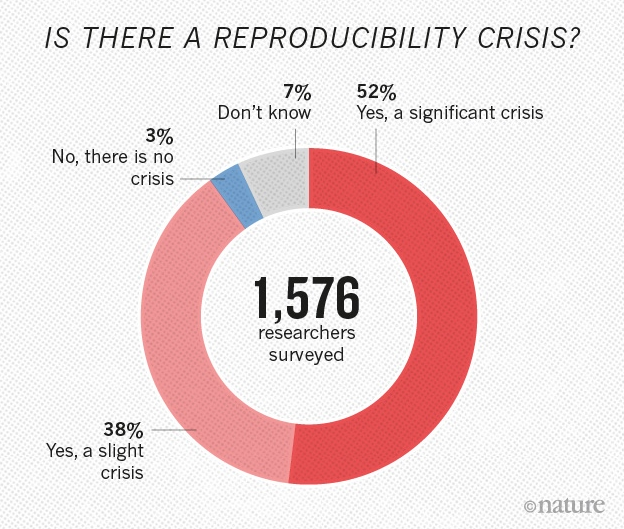
\includegraphics[width=0.45\textwidth,height=\textheight]{graphics/rep_crisis.png}
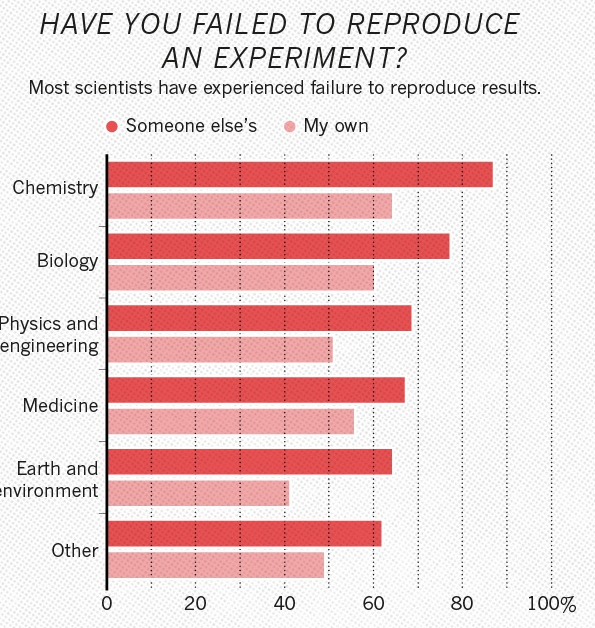
\includegraphics[width=0.45\textwidth,height=\textheight]{graphics/failed.png}
\end{frame}

\begin{frame}

\includegraphics{graphics/reproducibility.png}
\end{frame}

\begin{frame}
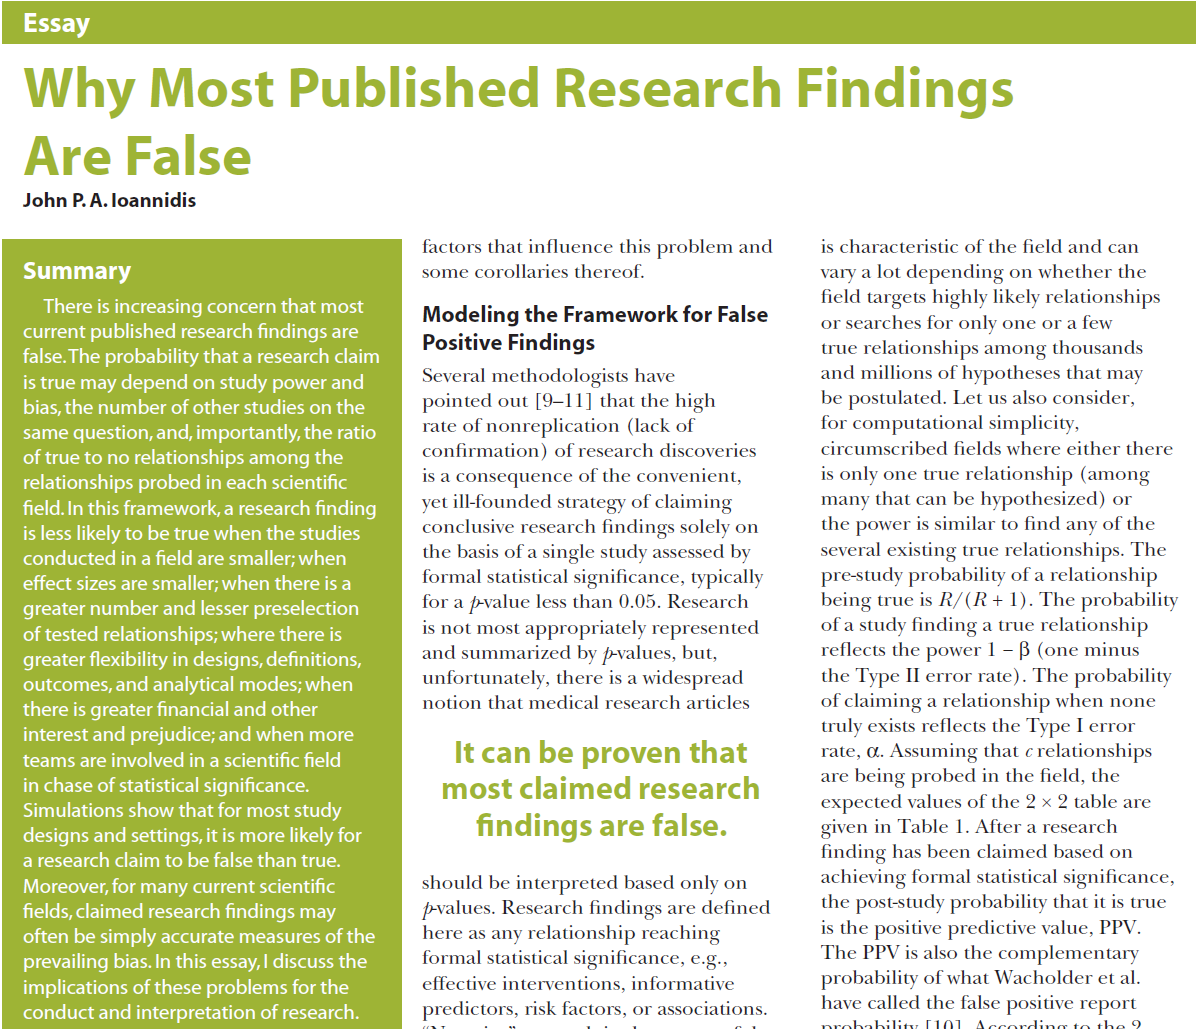
\includegraphics[width=0.6\textwidth,height=\textheight]{graphics/Ioannidis2.png}
\includegraphics[width=0.4\textwidth,height=\textheight]{graphics/nuzzo.png}


\includegraphics[width=0.5\textwidth,height=\textheight]{graphics/dirtydozen.png}
\includegraphics[width=0.45\textwidth,height=\textheight]{graphics/against_ss.png}
\end{frame}

\begin{frame}{Open and reproducible research\ldots{}}
\protect\hypertarget{open-and-reproducible-research}{}
\(~\)

\begin{itemize}
\tightlist
\item
  \ldots benefits the researcher (easy to track what you did, modify
  analyses, builds trust in your work, increases citation rates etc).
\end{itemize}

\vspace{2mm}

\begin{itemize}
\tightlist
\item
  \ldots benefits the research community (others can build on your data,
  code and results).
\end{itemize}

\vspace{2mm}

\begin{itemize}
\tightlist
\item
  \ldots benefits society (more insight for money, more trustworthy
  results, more scientific progress).
\end{itemize}

\vspace{2mm}

\begin{itemize}
\tightlist
\item
  \ldots are thus \emph{basic skills any researcher in the future will
  HAVE to master}!
\end{itemize}
\end{frame}

\begin{frame}
\begin{block}{Other institutions are a step ahead}
\protect\hypertarget{other-institutions-are-a-step-ahead}{}
\(~\)

For example, the Center for Reproducible Science, University of Zurich:

\(~\)

\url{https://www.crs.uzh.ch/en.html}
\end{block}
\end{frame}

\begin{frame}
\begin{block}{Our idea}
\protect\hypertarget{our-idea}{}
\(~\)

Given the positive feedback on the mentioned course (and the negative
feedback on other TS courses) and the importance of the topic, we
wondered:

\(~\)

\begin{itemize}
\tightlist
\item
  Is it possible to set up a transferable skills course at the
  department/faculty/entire NTNU?
\end{itemize}

\(~\)

\begin{itemize}
\tightlist
\item
  If yes, what would be the strategy forward?
\end{itemize}
\end{block}
\end{frame}

\end{document}
